\section*{Response to Reviewer 2}\label{par:r2}

{\large

\noindent \underline{\textbf{Comments:}}

The paper "FishboneChain" presents a blockchain architecture that enhances scalability and liquidity in crowdsourcing. It uses a main chain for fund management and child chains for task processing, reducing the main chain’s load. Smart contracts manage tasks and payments efficiently, allowing users to lock funds once for multiple tasks. The system includes periodic settlements and a hybrid dispute resolution mechanism, improving security. Simulations show up to 100x throughput improvement while maintaining security and flexibility.But this article has the following problems and needs to be revised：

{\color{blue}
\noindent \underline{\textbf{Reply:}}

Thank you for carefully reading our response and revision and giving positive comments above.
}\\ %end of color

1. In the Abstract, the sentence ``This leads to significant portion of funds being locked...'' lacks the article ``a,'' which should be corrected to ``a significant portion.''

{\color{blue}
\noindent \underline{\textbf{Reply and Modification:}}

Thank you for identifying the missing article in the Abstract. We revise the sentence to "a significant portion of funds being locked...". Additionally, we also thoroughly proofread the entire paper to address other grammatical errors and typographical mistakes.
}\\ % end of color

2. In Section IV.C (Design Goals), the phrase ``The system’s performance must meet the following goals'' is grammatically incomplete without a colon; it should read ``following goals:''.

{\color{blue}
\noindent \underline{\textbf{Reply and Modification:}}

We appreciate your attention to detail regarding the punctuation in Section IV.C. The sentence is amended to include a colon, reading ``following goals:'' as suggested.
}\\ % end of color

3. In Section VI.B (Fund Security),The sentence says, ``The financial loss for each participate is limited.'' The correct word should be ``participant'', not ``participate,'' which is a verb. This is a straightforward grammar mistake that undermines the professionalism of the writing.

{\color{blue}
\noindent \underline{\textbf{Reply and Modification:}}

Thank you for pointing out the incorrect word usage in Section VI.B. We replace ``participate'' with ``participant'' to ensure grammatical accuracy.
}\\ % end of color


4. While Figure 7 presents important data on the platform's performance as the main chain’s TPS increases, the main text fails to adequately explain the figure. No axis labels or legends are interpreted clearly, and readers are left to guess what the plotted data signifies. This weakens the impact of the results and makes it hard to validate the performance claims.

{\color{blue}
\noindent \underline{\textbf{Reply:}}

Thanks for your valuable suggestions. We acknowledge that the explanation of Figure 7 in our paper is inadequate, particularly regarding the axis, labels, legend descriptions, and experimental objectives. We revise these elements to provide a clearer presentation of the experimental data and better demonstrate the significance of this investigation. 

\noindent \underline{\textbf{Modification:}}

\renewcommand{\thefigure}{7}
\begin{figure}[htbp]
	\centering
	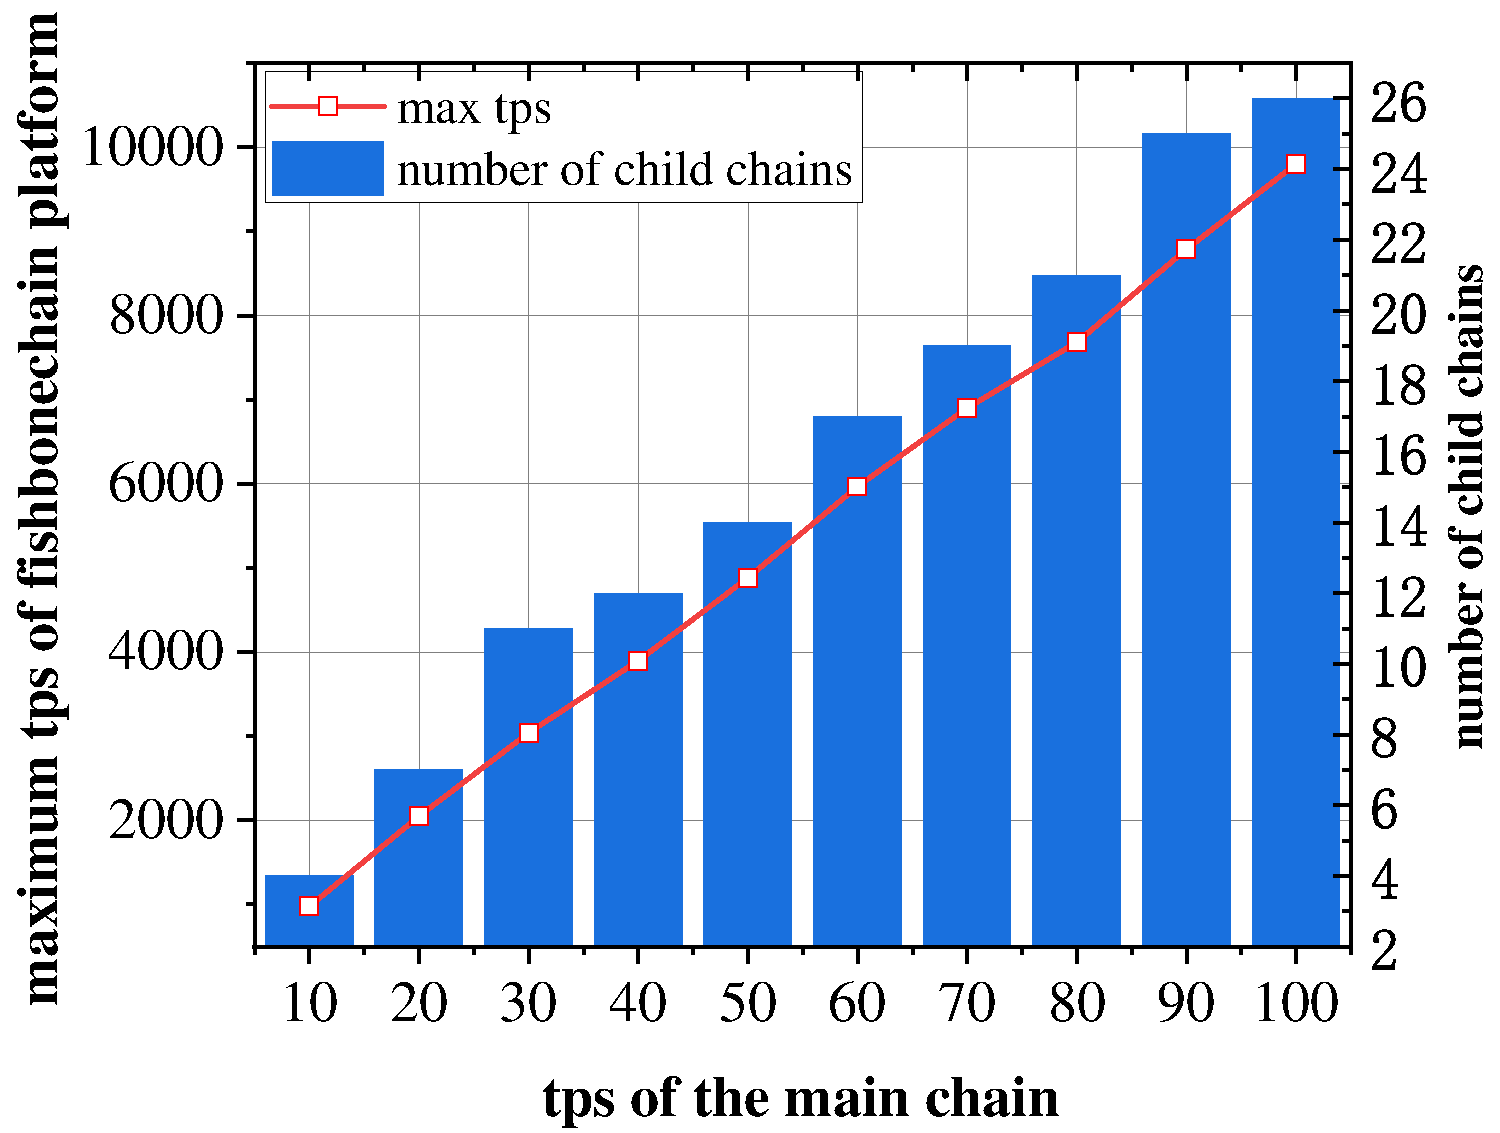
\includegraphics[width=0.55\linewidth]{Round-2/response/figures/max-tps.pdf} 
	\caption{Platform performance when tps of the main chain increase} 
	\label{fig:max_tps} 
\end{figure} 

After reaching around 1100 transactions per second, the tps of the main chain becomes the primary bottleneck, limiting the overall throughput of our platform. In the meantime, with the continuous development and maturation of technologies such as sharding, the tps of the main chain is expected to improve. To thoroughly investigate the maximum throughput potential of the platform system, we set the main chain tps within the range of 10-100 and conduct experiments to determine the maximum number of supported child chains and the corresponding total throughput under various main chain tps conditions. As shown in Fig.~\ref{fig:max_tps}, as the main chain tps continues to increase, the number of child chains and the maximum tps of the platform also increases linearly. When the main chain tps reaches 100, the platform can support 25 child chains and the maximum tps of the platform is reaching around 10000. These results demonstrate that our platform possesses significant performance scalability potential. Even a modest increase in the main chain's tps can facilitate the addition of multiple child chains, resulting in a substantial boost to the platform's overall throughput, potentially by several thousand. This underscores the platform's efficient architecture and its capacity for considerable expansion with relatively minor enhancements to the main chain's performance. Fig.~\ref{fig:max_tps} serves as a crucial reference framework for the architectural design and scalability planning of real-world crowdsourcing platforms. This performance mapping provides platform architects with precise guidance on system configuration requirements. For instance, when a platform's anticipated transaction volume approaches 10,000 transactions per second, our results demonstrate that maintaining a main chain processing capacity of at least 100 tps is essential to ensure operational stability and service quality. This insight is particularly valuable for large-scale crowdsourcing platforms with user bases in the millions, where transaction demands can fluctuate dramatically. The architectural flexibility illustrated in our results enables significant economic advantages through resource optimization. Platform designers can implement a cost-effective scaling strategy by maintaining moderate main chain performance while dynamically adjusting the number of child chains to accommodate changing demands. Furthermore, our architecture provides a progressive scaling pathway suitable for platforms at various growth stages. Emerging crowdsourcing applications can begin with minimal configurations, like lower main chain tps and fewer child chains, and scale incrementally as their user base expands. 
}\\ %end of color

5. The discussion of fund locking and liquidity in the ``Analyse of Fund Management Scheme" section is based on symbolic parameters like $t$, $b$, and $s$, but no real-world values or case studies are provided. How these variables translate to actual crowdsourcing platforms or real currency values. This limits the practical interpretability and weakens the section’s ability to demonstrate financial efficiency in realistic scenarios.

{\color{blue}
\noindent \underline{\textbf{Reply:}}

Thank you for your insightful feedback on the ``Analyse of Fund Management Scheme". To demonstrate the superiority of our periodic fund settlement scheme over the baseline approach that the user must lock the entire budget at the beginning of the task, we design a simplified scenario including parameters of $t$, $b$ and $s$.  In this experiment, the requester posts a task on each of $s$ child chains, with each task lasting $t$ epochs and requiring a budget $b$ per epoch. For analytical clarity, in the periodic scheme, the requester locks funds incrementally in $s$ steps, with each lock amount being $t*b$, while in the basic scheme, the requester must lock the entire budget ($s*t*b$) at the beginning of the tasks. Our previous explanation of these parameters is insufficient. We revise the ``Analyse of Fund Management Scheme" section to provide a more comprehensive interpretation of how these parameters function within our crowdsourcing environment.

\noindent \underline{\textbf{Modification:}}

\renewcommand{\thefigure}{8}
\begin{figure}[htbp]
    \centering
    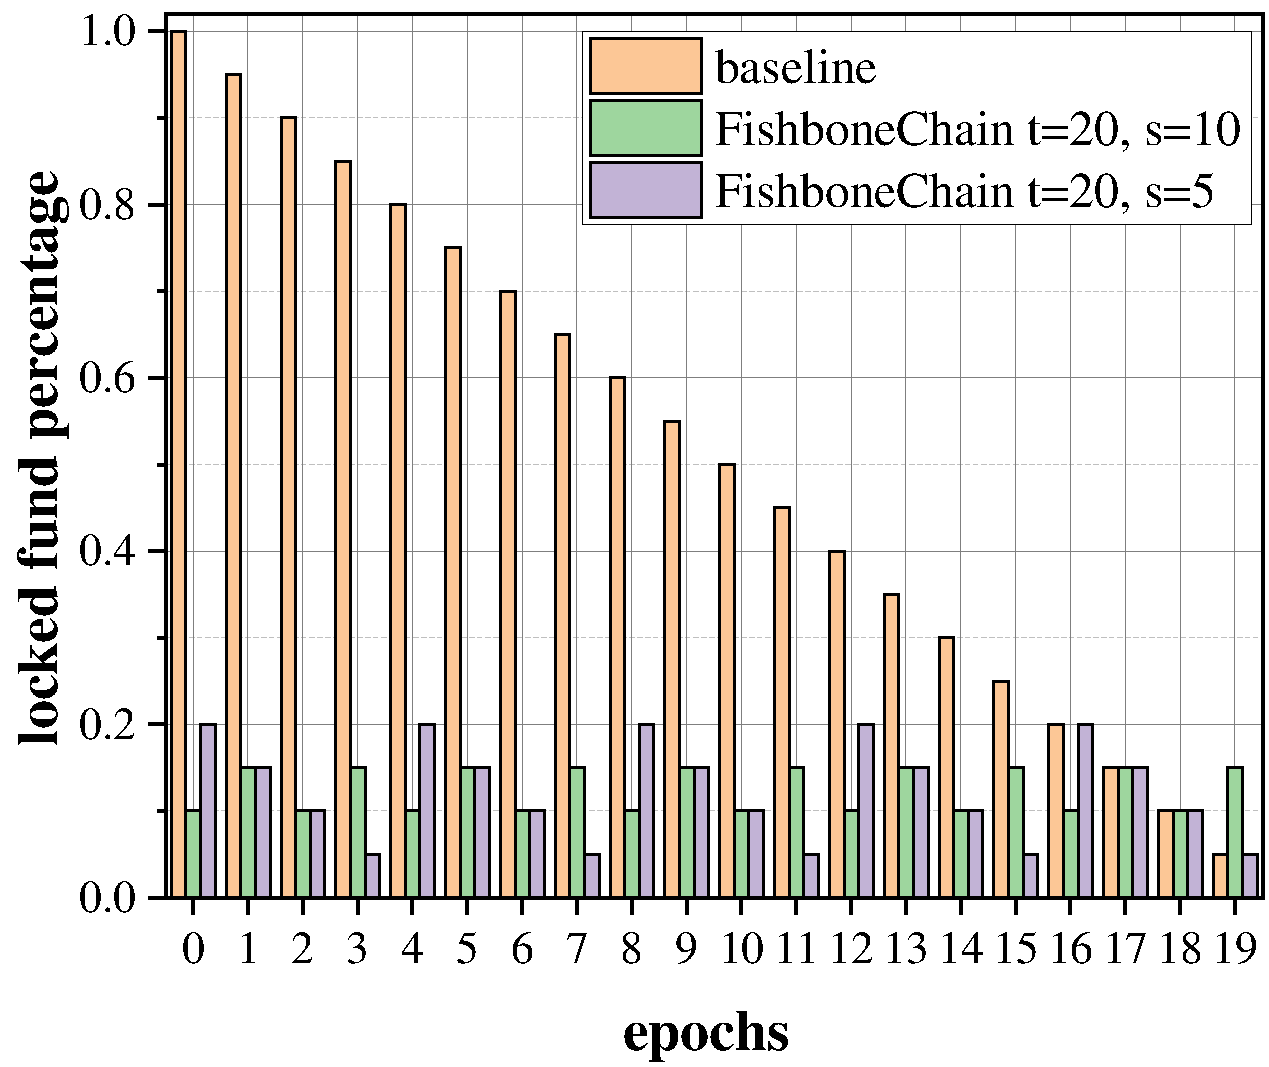
\includegraphics[width=0.55\linewidth]{Round-2/response/figures/locked_fund_comparison.pdf}
    \caption{Comparison of the percentage of locked funds}
    \label{fig:locked_fund_per}
\end{figure}

Next, we analyze the advantages of periodic fund management over the traditional approach. In the baseline scheme, requesters are required to lock individual budgets at the beginning of the task, leading to a potentially substantial accumulation of frozen funds. By contrast, our FishboneChain architecture permits requesters to periodically transfer funds to FMC for budget management, mitigating the locked fund issue. To compare locked fund percentages between the two schemes during task execution, we design a simplified periodic fund management mechanism. Assuming there are $s$ child chains with the same duration of epoch and a requester posts a task on each of them. Each task demands $t$ epochs for completion, and the budget per task is $b$. For the baseline, the requester should lock $L=tb$ for every task separately, which is a $s*t*b$ for frozen funds. For the baseline scheme, the requester needs to lock $L = tb$ funds for each task separately, resulting in a total initial locked amount of $L_{total} = s * L = s * t * b$. In the $i$-th period of $t$ periods, where $i \in [0,t)$, the frozen fund for each task is $F^{baseline}_i = (t-i)b$. In other words, at period $i=1$, the budget of each $T_i$ that is actively used is only $b$, while the remaining $F^{baseline}_1 = (t-1)b$, although not yet used, remains locked. At period $i=2$, the frozen fund for each task is $F^{baseline}_2 = (t-2)b$. At the last period ($i=t$), the frozen fund becomes $F^{baseline}_t = (t-t)b=0$, meaning all budgets are used in this period. Therefore, in the $i$-th period, the proportion of frozen funds in the total budget is $\frac{s*F^{baseline}_i}{s*L} = \frac{(t-i)b}{tb} = \frac{t-i}{t}$. Because the base scheme locks funds on the main chain, each is $tb$. For the convenience of analysis, in our scheme, the requester also locks the same fund $L=tb$ to the main chain at one time but periodically locks these funds in $s$ times. Therefore, at the $i$ epoch, $i \in [0,t)$, the total amount of locked funds is $F^{FishboneChain}_i= tb * (1+ \lfloor \frac{1}{t/s} \rfloor) $ and the total amount of used funds is $i * sb$. Therefore, the locked fund percentage in the $i$ epoch is $\frac{F^{FishboneChain}_i}{i * sb}=[t/s * (1+ \lfloor \frac{1}{t/s} \rfloor) - i]/{t}$.

As shown in Fig.~\ref{fig:locked_fund_per}, the percentage of locked funds is shown for the baseline and our scheme, where two sets of parameters are set for our simplified Fishbonechain scenario. The orange bar represents the baseline scheme, where the requester locks all budgeted funds on the blockchain at the beginning of the task. The green bar illustrates the scenario where the requester publishes 10 tasks on child chains, with each task requiring 20 epochs to complete. The purple bar depicts the scenario of 5 tasks posted on child chains, with each task also requiring 20 epochs for completion. The horizontal axis represents the current period, while the vertical axis shows the percentage of locked funds. It is clear that the percentage of locked funds in our scheme is consistently lower than the baseline scheme, which means that the funds are quickly applied to the task budget for the next epoch. Even if we adjust the number of tasks posted by the requester from 10 to 5, the percentage of locked funds is still less than or equal to $20 \%$. For example, in a data annotation project with 10 child chains, 20 epochs per task, and a \$500 budget per epoch, traditional schemes require locking \$100,000 upfront, while our periodic fund management scheme releases funds gradually. At 25\% completion, our approach only reserves \$15,000-\$20,000 compared to \$75,000 in the traditional approach, freeing substantial capital for other operations. Even in this simplified scenario, implementing a periodic fund management scheme significantly reduces requesters' financial burden. In practical applications with varying task quantities and epoch requirements, requesters can develop fine-grained strategies tailored to their specific needs. This reduced liquidity pressure enables requesters to post more tasks with the same amount of funds, collecting information more comprehensively. The resulting increased platform activity attracts more miners and workers, fostering a positive ecosystem cycle for our Fishbonechain platform.
}\\ %end of color

6. Several important figures like Fig. 7 and Fig. 8 are not discussed in sufficient depth in the main body. For instance, Fig. 8 compares locked fund percentages but the implications for real-world liquidity and capital efficiency are not analyzed.

{\color{blue}
\noindent \underline{\textbf{Reply:}}

Thank you for your valuable suggestions. We acknowledge that our analysis of Fig. 7 and Fig. 8 in the previous paper lacks sufficient depth. We provide a more thorough and detailed discussion in the revised paper, elaborating on the practical implications of these figures within the crowdsourcing text.
For Fig. 7, we now demonstrate how our scalability results directly translate to real-world deployment decisions, offering concrete guidelines for infrastructure investment and capacity planning based on anticipated transaction volumes. For Fig. 8, we enhance our analysis to show how the locked fund percentage metrics translate to tangible liquidity benefits and capital efficiency gains that can significantly impact operational costs and platform sustainability in production environments.

\noindent \underline{\textbf{Modification:}}

For \textbf{Fig. 7}, we add
``
Fig.~\ref{fig:max_tps} serves as a crucial reference framework for the architectural design and scalability planning of real-world crowdsourcing platforms. This performance mapping provides platform architects with precise guidance on system configuration requirements. For instance, when a platform's anticipated transaction volume approaches 10,000 transactions per second, our results demonstrate that maintaining a main chain processing capacity of at least 100 tps is essential to ensure operational stability and service quality. This insight is particularly valuable for large-scale crowdsourcing platforms with user bases in the millions, where transaction demands can fluctuate dramatically. The architectural flexibility illustrated in our results enables significant economic advantages through resource optimization. Platform designers can implement a cost-effective scaling strategy by maintaining moderate main chain performance while dynamically adjusting the number of child chains to accommodate changing demands. Furthermore, our architecture provides a progressive scaling pathway suitable for platforms at various growth stages. Emerging crowdsourcing applications can begin with minimal configurations, like lower main chain tps and fewer child chains, and scale incrementally as their user base expands. ''


For \textbf{Fig. 8}, we add
``
For example, in a data annotation project with 10 child chains, 20 epochs per task, and a \$500 budget per epoch, traditional schemes require locking \$100,000 upfront, while our periodic fund management scheme releases funds gradually. At 25\% completion, our approach only reserves \$15,000-\$20,000 compared to \$75,000 in the traditional approach, freeing substantial capital for other operations. Even in this simplified scenario, implementing a periodic fund management scheme significantly reduces requesters' financial burden. In practical applications with varying task quantities and epoch requirements, requesters can develop fine-grained strategies tailored to their specific needs. This reduced liquidity pressure enables requesters to post more tasks with the same amount of funds, collecting information more comprehensively. The resulting increased platform activity attracts more miners and workers, fostering a positive ecosystem cycle for our Fishbonechain platform.''
} %end of color

}